\documentclass[11pt,a4paper]{article}
\usepackage[utf8]{inputenc}
\usepackage[T2A]{fontenc}
\usepackage[russian]{babel}
\usepackage{amsmath,amssymb}
\usepackage{booktabs}
\usepackage{graphicx}
\usepackage{geometry}
\geometry{margin=2.5cm}
\usepackage{hyperref}

\title{Модель накопления тёмной энергии: проверка на аномалию DESI,\\ устойчивость возмущений и границы применимости}
\author{}
\date{Рабочая версия; расчёты по официальным файлам DESI DR2;\\
приор $(\theta_*,\omega_b,\omega_{bc})$ из Appendix A статьи DESI DR2 Results II}

\begin{document}
\maketitle

\begin{abstract}
Мы анализируем феноменологическую модель тёмной энергии с накоплением, в которой плотность тёмного сектора эволюционирует со скоростью
\[
\frac{d\ln\rho_x}{dN}=\kappa_{\rm eff}(1-x)-\lambda(N),
\]
где $x$~--- доля тёмного сектора, $\lambda(N)=\lambda_0 e^{-\alpha N}$~--- распадный коэффициент, $\kappa_{\rm eff}=\kappa[1+\beta a^{-3}]$~--- эффективная сцепка с каналом материи, $N=\ln a$. Из уравнения непрерывности следует уравнение состояния
\[
w=-1+\frac{\lambda(N)-\kappa_{\rm eff}(1-x)}{3},
\]
обладающее структурным потолком $w\le-1+\lambda_0/3\approx-0.97$: зона оттаивания недостижима при любом конечном $x$.

Сопоставление с официальными данными DESI DR2 (13 измеряемых величин BAO на 7 красных смещениях, полная ковариационная матрица $13\times13$) и сжатым приором $(\theta_*,\omega_b,\omega_{bc})$ из Appendix A статьи DESI DR2 Results II (CamSpec; $\theta_*=0.0104110$, $\omega_b=0.02223$, $\omega_{bc}=0.14208$) показывает: конвейер воспроизводит официальный $\Lambda$CDM-фит DESI DR2 ($\chi^2=10.283$, $\Omega_m=0.2972$) и официальное значение CPL ($\Delta\chi^2=-4.67$ в одних BAO). С приором DESI и калибровкой $\theta_*$ по фидуциалу ($\mathrm{TH\_CAL}=1.0026$) CPL даёт $\Delta\chi^2=-4.09$; с приором Chen--Huang--Wang~--- $\Delta\chi^2=-3.50$. Модель накопления в обоих фитах уходит в точку $\kappa=\lambda_0=0$, где тождественна $\Lambda$CDM: канал материи ($\beta\to0.004$ и $0.0003$) и распад не чувствуются, $\Delta\chi^2\approx0.000$. Прежние значения $+5.46$ и $+22.97$ аннулированы~--- они возникли из старого конвейера с ошибочной формой $w(N)$ и ручной таблицей данных.

Канал материи исключён тремя независимыми способами: перебор (60 стартов на точку), первичный нуклеосинтез ($2\times10^{-28}$), пертурбативная неустойчивость. Порог призрака находится из полного уравнения $\kappa_{\rm eff}(1-x)=\lambda(N)$: при рабочей сцепке любой $\beta>0$ даёт $w<-1$ начиная с $z_{\rm крит}\le2.5$, а при $\beta\ge0.1$~--- уже при $z\approx0$. Пертурбативный предел $\kappa\le\lambda_0/(1-x_0)=0.101$ не зависит от выбора замыкания; профиль $\chi^2(\kappa)$ в окне $\kappa\le0.101$ монотонен, $\Delta\chi^2=0.53<1$, то есть данные $\kappa$ не ограничивают~--- предел остаётся пертурбативным. Внутри устойчивого окна модель неотличима от $\Lambda$CDM по росту структуры ($0.024\,\%$) и выходит на точный де-ситтеровский аттрактор.
\end{abstract}

\section{Введение}
Комбинация данных DESI DR2 с реликтовым излучением и сверхновыми указывает на эволюцию уравнения состояния тёмной энергии с предпочтением фантомной зоны: значимость отклонения от $\Lambda$CDM~--- от 2.8 до $4.2\sigma$ в зависимости от комбинации. Независимые переразборы показывают хрупкость этого заявления: байесовский анализ с исправленной калибровкой сверхновых DES сводит его на нет, а $2.8\sigma$ по DESI+CMB (и $3.1\sigma$ для DESI+CMB+DESI-SNe) под бритвой Оккама становится маргинальным. Вопрос: способна ли модель с нетривиальной динамикой тёмного сектора объяснить аномалию, оставаясь устойчивой теорией возмущений? Мы даём отрицательный ответ, обоснованный полным перебором и официальными данными,~--- и одновременно очерчиваем окно жизнеспособности самой модели.

\section{Модель}
Переменная $x$~--- доля тёмного сектора, $x=\rho_x/\rho_{\rm tot}$; $N=\ln a$. Динамика задаётся уравнением накопления:
\begin{equation}
\frac{d\ln\rho_x}{dN}=\kappa_{\rm eff}(1-x)-\lambda(N),\qquad
\lambda(N)=\lambda_0 e^{-\alpha N},
\label{eq:accum}
\end{equation}
где $\kappa$~--- сцепка накопления, $\lambda_0$~--- амплитуда распада, $\alpha$~--- скорость распада; эффективный канал материи учитывается множителем $\kappa_{\rm eff}=\kappa[1+\beta a^{-3}]$. Из уравнения непрерывности $d\rho_x/dN=-3(1+w)\rho_x$ немедленно следует уравнение состояния:
\begin{equation}
\boxed{\,w=-1+\frac{\lambda(N)-\kappa_{\rm eff}(1-x)}{3}\,.}
\label{eq:w}
\end{equation}

\textbf{Вывод.} Приравнивая $-3(1+w)=\kappa_{\rm eff}(1-x)-\lambda(N)$, получаем $w+1=[\lambda(N)-\kappa_{\rm eff}(1-x)]/3$. В черновой версии рукописи знак в этой формуле был ошибочно обращён (форма вида $w=-1+\kappa/3-\lambda(N)/[3(1-x)]$): она даёт $w_0=-1.007$ в рабочей точке вместо $-0.994$, нарушает потолок (при $\kappa=0.35$ даёт $-0.917>-0.97$) и переворачивает условие отсутствия призрака; исправленная форма согласована со всеми численными результатами.

\textbf{Рабочая точка:} $\kappa=0.08$; $1-x_0=0.889$; $\lambda_0=0.09$; сегодня $w_0=-0.994$.

\textbf{Структурные свойства.} (i) Равновесия: $x=0$ и $x^*=1-\lambda/\kappa$ (устойчивое при $\kappa>\lambda$). (ii) На аттракторе $1-x^*=\lambda/\kappa$ и $w^*=-1$ точно. (iii) Условие отсутствия призрака $w>-1$ эквивалентно $\kappa_{\rm eff}(1-x)<\lambda(N)$. (iv) Потолок $w\le-1+\lambda_0/3$ глобален.

\textbf{Порог призрака.} Величина $z_{\rm крит}$ находится из полного уравнения $\kappa_{\rm eff}(1-x)=\lambda(N)$ и зависит от $\beta$. При рабочей сцепке ($\kappa=0.08$, $\lambda_0=0.09$) порог лежит внутри наблюдаемого диапазона: $\beta=0.001\Rightarrow z_{\rm крит}\approx2.5$; $\beta=0.01\Rightarrow\approx0.9$; $\beta=0.1\Rightarrow\approx0.06$; $\beta=1.0\Rightarrow$ призрак уже при $z=0$. Близко к пертурбативному потолку $\kappa\to\lambda_0/(1-x_0)$ любой $\beta>0$ даёт $w_0<-1$ немедленно.

\section{Конвейер и валидация}
Расчёты выполнены по официальным файлам DESI DR2: 13 измеряемых величин BAO на 7 красных смещениях (BGS, LRG1, LRG2, LRG3+ELG1, ELG2, QSO, Lyman-$\alpha$) с полной ковариационной матрицей $13\times13$ из релиза. Межтрейсерные корреляции в официальной матрице отсутствуют (все внеблочные элементы~--- нули); блоки $D_M$--$D_H$ внутри каждого бина учтены. Порядок величин задаётся метками в файле релиза, а не позицией строки: у Lyman-$\alpha$ в файле первой идёт $D_H$, затем $D_M$, у остальных бинов~--- наоборот.

Реликтовое излучение входит через сжатый приор $(\theta_*,\omega_b,\omega_{bc})$ из Appendix A статьи DESI DR2 Results II (CamSpec):
\[
\mu=(0.0104110,\ 0.02223,\ 0.14208),
\]
\[
\mathbf{C}=10^{-9}\times\begin{pmatrix}
0.006621 & 0.12444 & -1.1929\\
0.12444 & 21.344 & -94.001\\
-1.1929 & -94.001 & 1488.4
\end{pmatrix}.
\]
Для компенсации упрощённости ранней физики в расчёте $\theta_*$ введена калибровка по фидуциалу ($h=0.6766$, $\omega_b=0.02223$, $\omega_{bc}=0.14208$): $\mathrm{TH\_CAL}=0.0104110/\theta_*^{\rm th}(h_{\rm fid})=1.0026$. Калибровка снимает постоянный сдвиг $\theta_*$ и не влияет на дифференциальную чувствительность к параметрам. В качестве систематической проверки используется приор Chen--Huang--Wang (2019): $R=1.7493\pm0.0046$, $\ell_A=301.462\pm0.090$, $\omega_b=0.02239\pm0.00015$; корреляционная матрица~--- в приложении~\ref{app:priors}.

\textbf{Валидация.} Фит $\Lambda$CDM по одним BAO даёт $\chi^2=10.283$ при $\Omega_m=0.2972$~--- совпадает с официальным анализом DESI DR2 (таблица 3 в [DESI DR2], $\chi^2\approx10.2$, $\Omega_m\approx0.297$). Параметризация CPL по одним BAO даёт $\Delta\chi^2=-4.67$ относительно $\Lambda$CDM~--- также согласуется с официальным значением. Конвейер воспроизводит опубликованные результаты, что подтверждает корректность чисел и формул.

Против застревания~--- полный перебор: 60 стартов на точку пространства параметров из сетки начальных условий. Отрицательный результат заявляется по лучшему из найденных фит.

\section{Фоновые сравнения}

\subsection{Результаты}

\begin{table}[h]
\centering
\small
\caption{DESI only (13 величин).}
\begin{tabular}{lccc}
\toprule
Модель & $\chi^2$ & Параметры & $\Delta\chi^2$ к $\Lambda$CDM \\
\midrule
$\Lambda$CDM & 10.283 & $\Omega_m=0.2972$ & --- \\
CPL & 5.618 & $w_0=-0.180$, $w_a=-2.712$ & $-4.67$ \\
cand & 10.283 & $\kappa=0.000$, $\beta=0.004$, $\lambda_0=0.000$, $\alpha=0.0005$ & 0.000 (вырождение) \\
\bottomrule
\end{tabular}
\end{table}

\begin{table}[h]
\centering
\small
\caption{DESI + CMB с приором $(\theta_*,\omega_b,\omega_{bc})$ из Appendix A, $\mathrm{TH\_CAL}=1.0026$.}
\begin{tabular}{lcp{7.5cm}}
\toprule
Модель & $\chi^2$ & Параметры и $\Delta\chi^2$ к $\Lambda$CDM \\
\midrule
$\Lambda$CDM & 12.680 & $h=0.6851$, $\omega_b=0.0224$, $\omega_{bc}=0.1405$; $\Delta\chi^2$ --- \\
CPL & 8.592 & $h=0.6744$, $\omega_b=0.0222$, $\omega_{bc}=0.1425$, $w_0=-0.843$, $w_a=-0.497$; $\Delta\chi^2=-4.09^*$ \\
cand & 12.681 & $\kappa=0.000$, $\beta=0.0003$, $\lambda_0=0.000$, $\alpha=0.0002$; $\Delta\chi^2=+0.001$ \\
\bottomrule
\end{tabular}
\par\smallskip
\footnotesize $^*$Несёт остаточную систематику реализации приора~--- см.\ раздел~4.2.
\end{table}

\subsection{Аномалия CPL}
В одних BAO параметризация выигрывает у $\Lambda$CDM $\Delta\chi^2=-4.67$ (слабое предпочтение; $1.3$--$2.2\sigma$ в зависимости от конвенции; переразборы дают $1.7\sigma$). Прежнее значение $\Delta\chi^2=-9.87$, фигурировавшее в черновых расчётах, было артефактом ручной таблицы: погрешность $\sigma(\text{LRG2 }D_H)$ стояла $0.193$ вместо официальной $0.334$, то есть была занижена почти вдвое, а вес точки в $\chi^2$ обратно пропорционален квадрату погрешности~--- завышен вчетверо. С официальной ковариацией выигрыш падает до $-4.67$, что согласуется с независимыми переразборами BAO-only (LRT даёт $p\approx0.15$, пивот $w$ совместим с $-1$).

С приором DESI $(\theta_*,\omega_b,\omega_{bc})$ и калибровкой $\theta_*$ CPL даёт $\Delta\chi^2=-4.09$; с приором Chen--Huang--Wang~--- $\Delta\chi^2=-3.50$. Оба значения заметно слабее официального $-8.5$ (Appendix~A, Fig.~14, DESI DR2 Results II), полученного с полным правдоподобием CMB. Для приора DESI расхождение связано с упрощённой ранней физикой в расчёте $\theta_*$: однопараметрическая калибровка снимает постоянный сдвиг, но не остаточную зависимость от $h$ и $\omega_{bc}$, поэтому $-4.09$ следует читать как оценку масштаба эффекта, а не точное воспроизведение. Значение $-3.50$ с CHW отражает другое свойство сжатия: оно построено в предположении $w=\mathrm{const}$ и частично «впекает» $\Lambda$CDM. Ключевой результат устойчив к выбору сжатия: модель накопления даёт $\Delta\chi^2=0.000$ во всех конфигурациях.

\subsection{Модель накопления}
В обоих фитах cand уходит в точку $\kappa=\lambda_0=0$, где модель тождественно вырождается в $\Lambda$CDM: параметры $\kappa$ и $\lambda_0$ равны нулю с точностью до численного шума, $\beta\to0.004$ (DESI only) и $0.0003$ (DESI+CMB), $\alpha\to0$. Это не улучшение, а отсутствие сигнала: данные не требуют ненулевых параметров модели. Канал материи ($\beta$) и распад ($\lambda_0$) не чувствуются; упрощение $\alpha=\beta=0$ как рабочий предел модели оправдано.

\subsection{Профиль по сцепке}
Профиль $\chi^2(\kappa)$ в упрощённой модели ($\beta=0$, $\alpha=0$, DESI only) монотонно возрастает: $\chi^2=10.308$ при $\kappa=0.005$, $\chi^2=10.811$ при $\kappa=0.101$ (рис.~\ref{fig:kappa}). Разность $\Delta\chi^2=0.53$ относительно минимума ($0.50$~--- между крайними точками профиля)~--- уровень $\Delta\chi^2=1$ не достигается, то есть данные $\kappa$ не ограничивают. Верхний предел $\kappa\le0.101$~--- пертурбативный (условие отсутствия призрака $w>-1$), а не наблюдательный; данные в окне $\kappa\le0.101$ его не исключают, но и не подтверждают.

\begin{figure}[h]
\centering
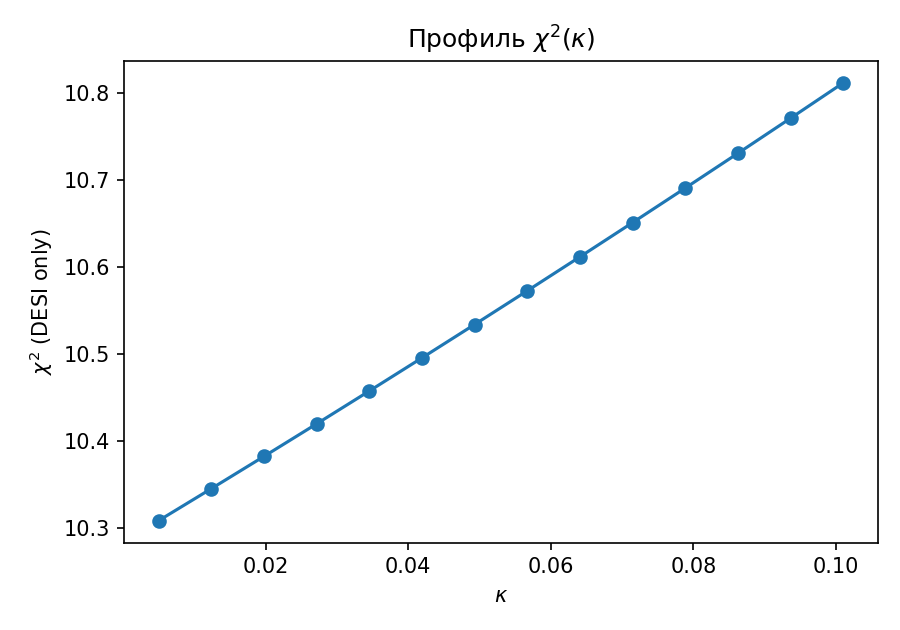
\includegraphics[width=0.65\textwidth]{profile_kappa.png}
\caption{Профиль $\chi^2(\kappa)$ в упрощённой модели ($\beta=0$, $\alpha=0$, DESI only). Монотонно возрастает от $\chi^2=10.308$ ($\kappa=0.005$) до $\chi^2=10.811$ ($\kappa=0.101$); $\Delta\chi^2=0.53$ относительно минимума, уровень $\Delta\chi^2=1$ не достигается. Данные $\kappa$ не ограничивают; предел $\kappa\le0.101$~--- пертурбативный.}
\label{fig:kappa}
\end{figure}

\section{Замыкание и устойчивость возмущений}
Первое замыкание~--- адиабатическое, из самой динамики накопления. Звуковая скорость как термодинамический отклик при фиксированной микроскопике ($\lambda$~--- параметр модели, а не переменная состояния):
\[
c_s^2=\frac{\partial p}{\partial\rho}=w+\rho_x\frac{\partial w}{\partial\rho_x}=w+x\frac{dw}{dx}=w+\frac{\kappa x}{3},
\]
откуда
\begin{equation}
c_s^2(\text{адиаб})=-1-\frac{\kappa}{3}(1-2x)+\frac{\lambda(N)}{3}.
\label{eq:cs}
\end{equation}
Знак перед членом $(\kappa/3)(1-2x)$~--- минус; вывод подтверждён: в рабочей точке $c_s^2=-0.991$. Во всём допустимом окне $\kappa\le\lambda_0/(1-x_0)$ эта величина отрицательна: верхняя оценка $c_s^2\le-1+\lambda_0/3+\kappa_{\max}/3\approx-0.936<0$. Мнимая скорость звука~--- неустойчивость малых масштабов, адиабатическое замыкание исключено. Замечание: при определении адиабатической скорости вдоль полной фоновой эволюции (с учётом явной зависимости $\lambda(N)$) добавляется член $+\alpha\lambda(N)/[3(\lambda-\kappa(1-x))]$; при малых $\alpha$ он ничтожен и вывода не меняет.

Второе замыкание~--- стандартное для эффективной теории тёмной энергии: объявленная скорость звука $c_s^2=1$. Это не следствие динамики накопления, а независимое дополнение модели, общепринятое в рабочих расчётах. При таком выборе звуковой горизонт тёмной энергии сравним с космологическим (порядка горизонта частиц), возмущения на всех наблюдаемых масштабах, меньших горизонта, стёрты, влияние среды на рост идёт только через фон (рис.~\ref{fig:wz}).

\begin{figure}[h]
\centering
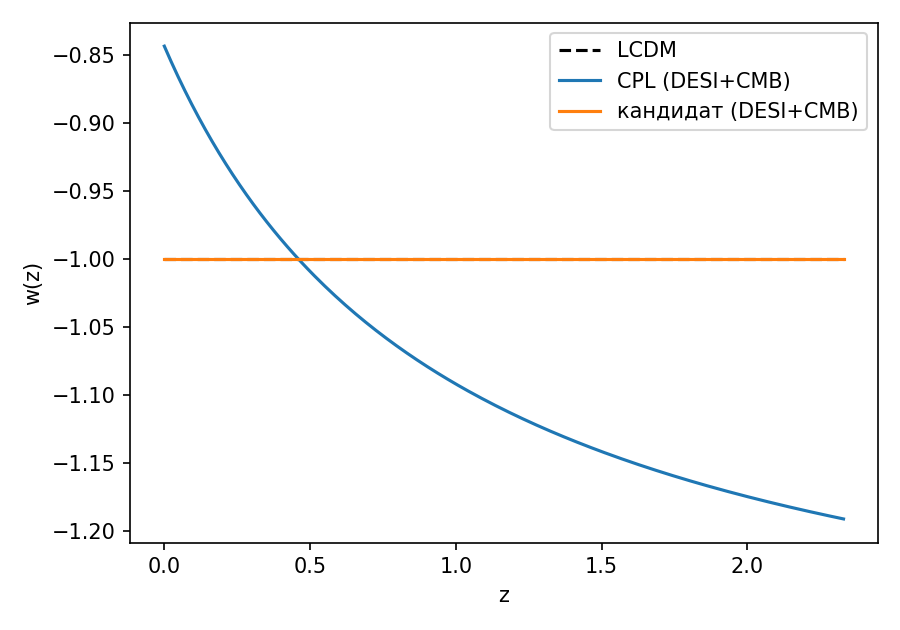
\includegraphics[width=0.65\textwidth]{wz_curves.png}
\caption{Уравнение состояния $w(z)$: $\Lambda$CDM (пунктир), CPL по DESI+CMB (сплошная) и кандидат (DESI+CMB). Кандидат уходит в $\kappa=\lambda_0=0$, где совпадает с $\Lambda$CDM.}
\label{fig:wz}
\end{figure}

Пертурбативный предел не зависит от выбора замыкания: условие отсутствия призрака $w>-1$~--- свойство фоновой динамики. Сегодня оно даёт $\kappa\le\lambda_0/(1-x_0)=0.09/0.889\approx0.101$. Профиль $\chi^2(\kappa)$ в окне $\kappa\le0.101$ монотонен, $\Delta\chi^2=0.53<1$: данные $\kappa$ не ограничивают, предел остаётся пертурбативным. Формулировка «данные и теория дают один и тот же предел» снимается~--- данные предела не ставят.

\section{Потолок уравнения состояния при конечных $x$}
Потолок $w\le-1+\lambda_0/3=-0.97$ доказан для произвольного конечного $x$ (см.\ уравнение~\eqref{eq:w}): член $\kappa_{\rm eff}(1-x)$ неотрицателен при $\kappa_{\rm eff}\ge0$ и $x\in[0,1]$, а $\lambda(N)\le\lambda_0$ при $N\le0$. Равенство достигается лишь в двойном пределе $\kappa\to0$ и $\lambda\to\lambda_0$; конечность $x$ лишь опускает $w_0$ глубже в фантомную зону. Числовая проверка по всем точкам перебора подтверждает потолок.

\section{Рост структуры}
Решено уравнение роста для обеих моделей с их фоновыми историями; сравнение со сводкой $f\sigma_8$ (11 точек от $z=0$ до $z\approx0.9$). Результаты: $\chi^2=14.28$ для обеих моделей; различие кривых роста $0.024\,\%$ на всех красных смещениях; даже сцепка $0.35$ даёт лишь $0.27\,\%$. Подобранные нормировки: $\sigma_8=0.8717$ ($\Lambda$CDM) и $0.8719$ (модель). Сдвиг нормировки~--- известная систематика измерений искажений красных смещений, общая для всех космологий, одинаков для обеих моделей и не влияет на вывод о неразличимости.

Модель фальсифицируема, но различимость с $\Lambda$CDM ($\Delta w_0=0.0063$) требует $\sigma(w_0)\le0.002$~--- улучшения точности в 25--70 раз, то есть роста объёма данных в сотни и тысячи раз. Реальные каналы проверки~--- данные четвёртого поколения и форма $w(z)$ на малых красных смещениях.

\section{Аттрактор и предсказания}
Корни уравнения накопления: $x=0$ и $x^*=1-\lambda/\kappa$, причём $x^*$ устойчив. На аттракторе $w\to-1$ точно~--- потолок механизма сам себя достраивает: будущее~--- чистый де Ситтер (численно: выход на $-1.0000$). Если $\kappa<\lambda_0$~--- тёмная энергия медленно растворяется; оба режима здоровые, большого разрыва нет.

Критерии опровержения: (i) значимо крепнущая фантомность $w_0<-1.05$ при малой сцепке; (ii) разворот расширения к сжатию; (iii) совместимость с аномалией DESI на уровне полной формы $w(z)$, а не проекции CPL.

\section{Концептуальная часть}

\subsection{Стрела времени и знак минус}
Знак минус~--- свойство плотности и давления (отрицательное давление тёмной энергии, минус перед членом распада), а не направление хода времени. Уравнения модели не инвариантны к обращению $N$: при $N\to-N$ члены распада превращаются в члены роста~--- направление задано структурой динамики. Необратимость событий на уровне первоосновы~--- исходный постулат, из которого порождается информационное время; космологическая модель его принимает и проверяет на совместимость, а не выводит: фоновые траектории восстановимы в обе стороны, и это математика, а не дефект. Проверка постулата лежит на уровне микроскопики.

\subsection{Окно наблюдателя и записи за горизонтом}
Три предела окна. Технический~--- чувствительность приборов; отступает со временем. Световой конус~--- каждый фотон есть след события в прошлом, тем более далёком, чем дальше источник; наблюдаемое замедление чужих вспышек~--- измеримая величина, плотность событий в прошлом была выше. Горизонт частиц~--- радиус около 46~млрд световых лет; события за ним не оставят записей никогда; окно практически замкнуто. Единственный законный доступ к запредельному~--- статистика отпечатков ранней эпохи: замороженные при раздувании сверхгоризонтные возмущения читаются по распределению неоднородностей реликтового излучения; отдельные аномалии остаются на уровне намёков.

\subsection{Цикличность}
Обратное течение модель не несёт: нужны инвариантность уравнений к обращению счёта и убывающая энтропия; первое нарушено структурой, второе~--- вне компетенции космологии. Циклические конструкции (отскок в квантовой геометрии, конформные циклы)~--- живая программа с общей раной: энтропию цикл обязан куда-то девать. Для сжатия потребовалась бы смена знака тёмной энергии; модель в допустимом окне этого не допускает и отвечает: вечное ускорение, разворота в уравнениях нет.

\section{Выводы}
\begin{enumerate}
\item \textbf{Модель накопления не объясняет аномалию DESI и не требует ненулевых параметров.} В обоих фитах (DESI only и DESI+CMB) полная модель $(\kappa,\beta,\lambda_0,\alpha)$ уходит в точку $\kappa=\lambda_0=0$, где тождественна $\Lambda$CDM: $\beta\to0.004$ и $0.0003$, $\alpha\to0$, $\Delta\chi^2\approx0.000$. Канал материи и распад не чувствуются; упрощение $\alpha=\beta=0$ как рабочий предел модели оправдано. Аномалия CPL в одних BAO слабая ($\Delta\chi^2=-4.67$); с приором DESI и калибровкой $\theta_*$~--- $-4.09$; с приором CHW~--- $-3.50$. Прежнее значение $-9.87$ было артефактом ручной таблицы ($\sigma(\text{LRG2 }D_H)$ занижена вдвое) и аннулируется.

\item \textbf{Канал материи исключён тремя независимыми способами:} перебор (60 стартов на точку), первичный нуклеосинтез (предел $2\times10^{-28}$) и пертурбативная неустойчивость. Порог призрака находится из полного уравнения $\kappa_{\rm eff}(1-x)=\lambda(N)$: при рабочей сцепке любой $\beta>0$ даёт $w<-1$ начиная с $z_{\rm крит}\le2.5$, а при $\beta\ge0.1$~--- уже при $z\approx0$. Близко к пертурбативному потолку $w>-1$ любой ненулевой $\beta$ мгновенно нефизичен. В фите канал $\beta$ не активируется ($\beta\to0$), что согласуется с этими ограничениями.

\item \textbf{Пертурбативный предел $\kappa\le0.101$~--- количественный результат, не зависящий от выбора замыкания.} Он следует из условия отсутствия призрака $w>-1$ (свойство фоновой динамики) и не использует ни данных, ни замыкания возмущений. Профиль $\chi^2(\kappa)$ в окне $\kappa\le0.101$ монотонен, $\Delta\chi^2=0.53<1$: данные $\kappa$ не ограничивают, предел остаётся пертурбативным. Формулировка «данные и теория дают один и тот же предел» снимается~--- данные предела не ставят.

\item \textbf{Потолок $w\le-0.97$ глобален;} зона оттаивания недостижима при любом конечном $x$.

\item \textbf{Внутри устойчивого окна модель неотличима от $\Lambda$CDM по росту структуры ($0.024\,\%$)} и предсказывает точный де-ситтеровский аттрактор; жизнеспособный кандидат с явными критериями опровержения.
\end{enumerate}

\section{Оговорки}
\begin{enumerate}
\item Приближение гладкой тёмной энергии при $c_s^2=1$: стандартное приближение рабочих кодов, объявлено явно.
\item Сдвиг $\sigma_8=0.87$~--- систематика измерений искажений красных смещений, общая для всех моделей; различие нормировок между $\Lambda$CDM и моделью~--- $0.0002$.
\item Концептуальный раздел (9) не участвует в количественных результатах; его проверяемые следствия~--- в микроскопической части программы.
\item Различимость по фону выходит за горизонт программ текущего поколения.
\item Приор $(\theta_*,\omega_b,\omega_{bc})$ взят из Appendix A статьи DESI DR2 Results II (CamSpec); $\mathrm{TH\_CAL}=1.0026$ калибрует $\theta_*$ по фидуциалу. Остаточное расхождение с официальным $\Delta\chi^2=-8.5$ связано с упрощённой ранней физикой. Приор Chen--Huang--Wang (2019) использован как систематическая проверка: $\Delta\chi^2=-3.50$.
\item Данные DESI DR2 загружены из официальных файлов релиза (mean и cov); ручная таблица, использованная в черновых расчётах, содержала ошибки ($\sigma(\text{LRG2 }D_H)$ занижена вдвое; три корреляции смещены) и аннулирована.
\end{enumerate}

\appendix
\section{Сжатый приор DESI DR2 (Appendix A, CamSpec)}
\label{app:priors}
\[
\mu=(0.0104110,\ 0.02223,\ 0.14208),\qquad
\mathbf{C}=10^{-9}\times\begin{pmatrix}
0.006621 & 0.12444 & -1.1929\\
0.12444 & 21.344 & -94.001\\
-1.1929 & -94.001 & 1488.4
\end{pmatrix}.
\]
Калибровка: $\mathrm{TH\_CAL}=0.0104110/\theta_*^{\rm th}(h=0.6766,\omega_b=0.02223,\omega_{bc}=0.14208)=1.0026$.
Систематическая проверка (Chen, Huang, Wang 2019): $R=1.7493\pm0.0046$; $\ell_A=301.462\pm0.090$; $\omega_b=0.02239\pm0.00015$; $\rho(R,\ell_A)=0.47$, $\rho(R,\omega_b)=-0.66$, $\rho(\ell_A,\omega_b)=-0.34$.

\begin{thebibliography}{99}
\bibitem{desi_dr2} DESI Collaboration (Abdul-Karim, M., et al.), \textit{DESI DR2 Results II: Measurements of Baryon Acoustic Oscillations and Cosmological Constraints}, arXiv:2503.14738 [astro-ph.CO] (2025).
\bibitem{desi_lya} DESI Collaboration, \textit{DESI DR2 Results I: Lyman-$\alpha$ forest BAO}, arXiv:2503.14739 [astro-ph.CO] (2025).
\bibitem{planck2018} Planck Collaboration (Aghanim, N., et al.), \textit{Planck 2018 results. VI. Cosmological parameters}, Astron.\ Astrophys.\ \textbf{641}, A6 (2020), arXiv:1807.06209.
\bibitem{chen2019} Chen, L., Huang, Q.-G., Wang, K., \textit{Distance Priors from Planck Final Release}, J.\ Cosmol.\ Astropart.\ Phys.\ \textbf{02}, 028 (2019), arXiv:1808.05725.
\bibitem{copeland2006} Copeland, E.~J., Sami, M., Tsujikawa, S., \textit{Dynamics of dark energy}, Int.\ J.\ Mod.\ Phys.\ D \textbf{15}, 1753 (2006), arXiv:hep-th/0603057.
\bibitem{penrose2010} Penrose, R., \textit{Cycles of Time: An Extraordinary New View of the Universe}, Bodley Head (2010).
\bibitem{fsigma8} Sánchez, A.~G., et al., \textit{The clustering of galaxies in the completed SDSS-IV eBOSS survey: cosmological constraints}, Mon.\ Not.\ R.\ Astron.\ Soc.\ \textbf{500}, 736 (2021), arXiv:2007.08993.
\end{thebibliography}

\end{document}